\chapter{The High Granularity Calorimeter}
\label{chap:hgcal}

\section{Introduction}
In order to fully exploit the physics potential of the LHC, 
the accelerator will be operated until around 2040 
in order to collect as much data as possible.
During this period, various upgrades are planned 
which are designed to maximise the instantaneous delivered to the experiments, including CMS.
As a result of this increase, and due to accumulated radiation damage, 
parts of the CMS detector will need to be upgraded.
A key part of this upgrade program is the replacement of the electromagnetic 
and hadronic calorimeter endcaps with the high granularity calorimeter (HGCAL).
In this chapter, the motivation for and design of the HGCAL is described.
The development of reconstruction software is detailed, 
and the detector's physics potential is demonstrated using the example of the VBF \Hgg analysis.

\section{The High Luminosity LHC}

Run~2 of the LHC is now complete, with over \SI{190}{\fbinv} of data delivered at $\sqrt{s}\,=\,\SI{13}{TeV}$. %original target was 150 Run 1 plus Run 2
This exceeds the original target of \SI{150}{\fbinv}, and was achieved partly because the machine was eventually operated at twice its nominal instantaneous luminosity.
The instantaneous luminosity reached values as high as \SI{2e34}{\lumi} during 2018.
The second long shutdown (LS2) commenced following the completion of Run~2 and will last until 2021.
During this time various improvements to the LHC will be made, including a substantial upgrade to the injection system.
The machine will also be readied for operation at the increased energy of \SI{7}{TeV} per beam.
However these upgrades will not substantially affect the conditions experienced by the LHC experiments; 
the peak instantaneous luminosity is not envisaged to increase beyond \SI{2e34}{\lumi}.
As such no major changes are required to the CMS detector during LS2, although various improvements are planned: 
these include upgrades to the muon system and HCAL barrel.
Therefore the expectation for Run~3, which commences in 2021 with two years of high-availability data-taking in 2022 and 2023, 
is that a further $\SI{150}{\fbinv}$ of data will be accumulated. 
%See here for details of LS2 and Run 3: https://indico.cern.ch/event/773482/contributions/3213751/attachments/1763994/2863045/LHC-Run2.CMS.Dec18.JW.pdf

Beyond Run~3, the usefulness of running the LHC with its current parameters decreases.
In order to reduce the statistical error on physics measurements by a factor of two, high-availability operation for more than ten years would be required.
Therefore a major upgrade to the LHC is planned, referred to as the Phase~2 upgrade, to maximise its physics reach. 
%insert info about what is actually being upgraded here? %TODO learn a bit about the things below 
%The technological innovations facilitating the upgrade include $\SI{12}{T}$ superconducting magnets, compact and precise superconducting cavities, and new beam collimation technology.
The resulting High~Luminosity~LHC (HL-LHC) \cite{HLLHC} will have a nominal levelled instantaneous luminosity of \SI{5e34}{\lumi}, 
permitting a total of \SI{3000}{\fbinv} of data to be collected by the mid-2030s.
The current planned schedule of the future running of the LHC and HL-LHC is summarised in Figure~\ref{fig:hgcal_LHCschedule}.

\begin{figure}[h!]
  \centering
  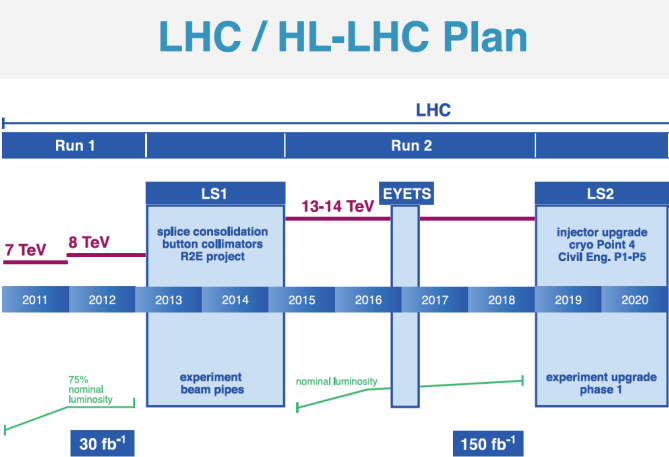
\includegraphics[width=0.8\textwidth]{Figures/HGCAL/LHCschedule1.png}
  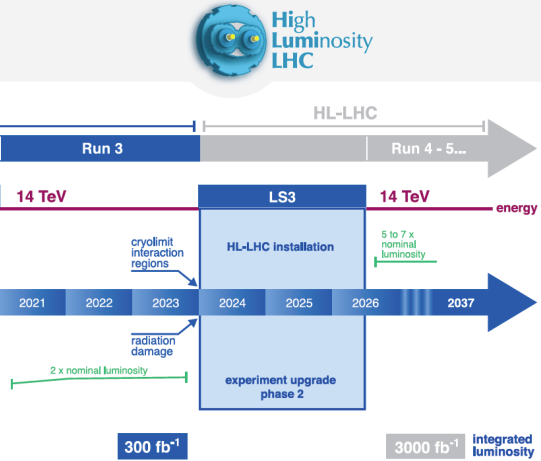
\includegraphics[width=0.8\textwidth]{Figures/HGCAL/LHCschedule2.png}
  \caption[Planned LHC and HL-LHC schedule.]
  {
    The planned schedule for the operation of the LHC and its high-luminosity upgrade.
    Figure taken from Ref.~\cite{FutureYR}.
  }
  \label{fig:hgcal_LHCschedule}
\end{figure}

\section{The CMS upgrade}

At the HL-LHC, the mean pileup per bunch crossing is expected to be 140; 
however an additional 50\% beyond the nominal value is allowed for in the HL-LHC design, 
which would result in mean pileup values of up to 200.
This constitutes a major change, and the environment will be significantly harsher than with the current LHC conditions.
These conditions pose serious challenges to the detectors in terms of radiation tolerance and reconstruction in high pileup.
In order to maintain or improve upon the excellent performance exhibited in Run~2, a suite of upgrades to the CMS detector are planned.
The key aspects of the CMS Phase~2 upgrade can be summarised as \cite{UpgradeTP,MTD}:
\begin{itemize}
  \item{\textbf{Tracker:}
  the tracker will suffer significant radiation damage and must be entirely replaced for Phase~2.
  The upgraded tracker will have finer granularity, %factor of 4
  increased coverage in the forward region, %up to eta=4
  and be much lighter, resulting in a reduced material budget.
  Furthermore, the design will allow track information to be included in the L1 trigger decision.}
  %enabling powerful background rejection at the earliest event selection step
  \item{\textbf{Endcap calorimeters:}
  the calorimeter endcaps (both ECAL and HCAL) will also be radiation-damaged by the end of Run~3, and will therefore be replaced.
  The replacement design, known as the high granularity calorimeter (HGCAL), will have both electromagnetic and hadronic sections.
  Fine segmentation in each of the longitudinal and transverse directions will facilitate precise measurements of showers in three dimensions.}
  \item{\textbf{ECAL barrel:}
  the current ECAL detector electronics are not capable of meeting the stringent HL-LHC trigger requirements.
  The level of noise in the silicon avalanche photodiodes which detect the scintillation light will also increase due to radiation damage.
  Therefore the electronics will be optimised and the operating temperature of the system reduced.} % from 18 to 8 degrees
  \item{\textbf{Timing:}
  precision timing measurements of objects will be made with the HGCAL and the upgraded ECAL.
  In addition, a dedicated timing layer providing precise timing information for minimum ionising particles will be added to the barrel and each of the endcaps.
  By enabling the reconstruction of vertex times, this will greatly improve the capability for pileup rejection.}
  \item{\textbf{Muon endcaps:}
  the CSC muon system will be enhanced with additional stations.
  This will increase the forward coverage and maintain muon acceptance at the L1 trigger.}
  %because new bits provide redundancy (only 1.5 to 2.4 doesn't have redundancy in muon system atm) and timing resolution.
  \item{\textbf{Trigger and data acquisition:}
  due to the tracker upgrade, the latency of the L1 trigger at Phase~2 is increased to \SI{12.5}{\micro\second}.
  Combined with upgrades to the front-end electronics of various subdetectors, %barrel calorimeter; the CSCs of the inner rings, and the DT readout.
  this enables an increase of the L1 trigger acceptance rate to \SI{500}{\kilo\hertz}.
  Consequently the data acquisition system must also be upgraded to handle the increase in event rate, event size, and the complexity of high PU reconstruction.}
\end{itemize}
Full details of the CMS upgrade scheme can be found in Refs~\cite{Tracker_Phase2TDR,Barrel_Phase2TDR,Muon_Phase2TDR,Trigger_Phase2TDR,DAQ_Phase2TDR,MTD,HGCAL}.
The remainder of this chapter is dedicated to describing the HGCAL in further detail, based upon Ref.~\cite{HGCAL}.

\section{Requirements for the HGCAL}

The primary challenge which drives the design of the HGCAL is the need to 
sustain physics performance in the extremely high pileup conditions foreseen at the HL-LHC.
Simulations indicate that the HGCAL will be required to withstand up to 2MGy of total radiation dose, 
together with a maximum fluence of around $\SI{10e16}{\textrm{n}_{\textrm{eq}}/\textrm{cm}^2}.$
The inhomogeneous distribution of this dose is shown in Figure~\ref{fig:hgcal_Dose}, 
which illustrates how the radiation dose is greatest near the beampipe.
Studies performed in recent years have shown that silicon sensors and the associated electronics 
retain acceptable performance after exposure to this level of radiation, 
and have hence been chosen as the most reliable active material for the majority of the calorimeter.
The remaining parts of the detector in lower-radiation regions will instead use 
cheaper plastic scintillator tiles with silicon photomultiplier (SiPMs) readout.
These layers of active material are interleaved with the copper-tungsten alloy absorber 
in the front section of the calorimeter, and stainless steel absorber further back.

\begin{figure}[h!]
  \centering
  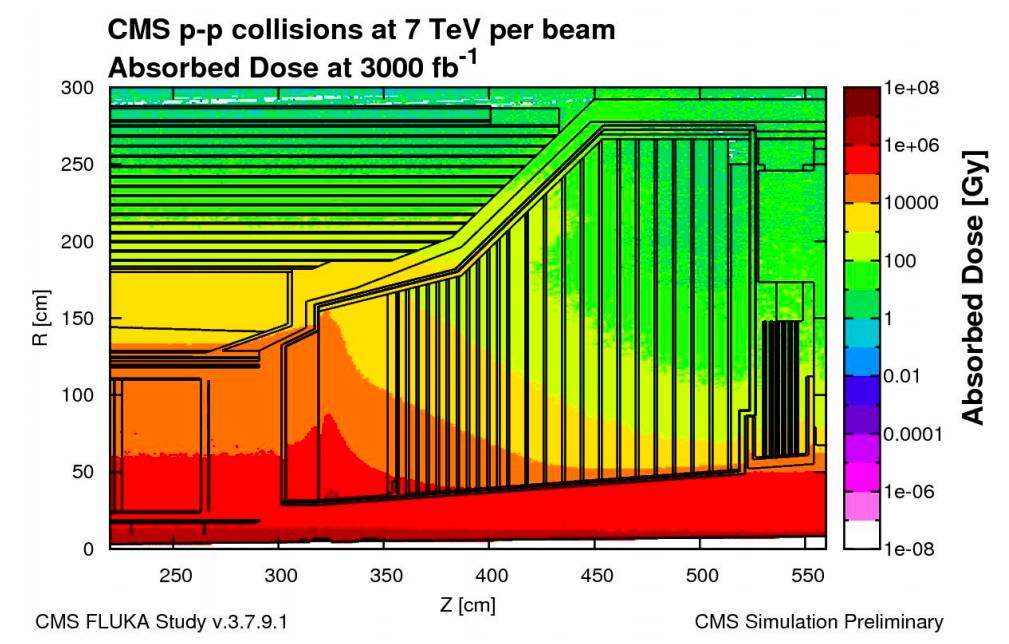
\includegraphics[width=\textwidth]{Figures/HGCAL/Dose.png}
  \caption[Expected radiation dose for the HGCAL.]
  {
    The dosage of ionising radiation the HGCAL is expected to absorb 
    after a total integrated luminosity of \SI{3000}{\fbinv}, 
    as a function of detector radius and depth.
    The colour scale indicates the magnitude of the absorbed dose.
    Figure taken from \cite{HGCAL}.
  }
  \label{fig:hgcal_Dose}
\end{figure}

To maintain performance throughout the operation of the HL-LHC it is necessary 
to inter-calibrate cells to the level of a few percent.
This is possible provided the signal-to-noise ratio (S/N) 
for minimum-ionising particles (MIPs) is sufficiently high.
For this to be achieved after \SI{3000}{\fbinv} of data has been collected, 
small silicon cells with low capacitance are required, which results in high lateral granularity.
Fine lateral granularity also has many benefits for physics performance, 
including the ability to separate nearby showers, identify narrow jets 
such as those originating from the quarks produced in vector boson fusion (VBF) events, 
and minimise the amount of pileup entering energy measurements.
To take advantage of this fine segmentation the calorimeter is required to be dense, 
thereby preserving the compactness of showers in the transverse direction.
Similarly, fine longitudinal granularity facilitates precise energy measurements, 
as well as enabling discrimination between different types of shower using the depth profile.
These features are particularly important 
within the CMS particle flow reconstruction paradigm \cite{ParticleFlow}.
A detector producing three-dimensional images of showers would provide 
powerful separation of electromagnetic, charged hadronic and neutral hadronic components,
facilitating more precise energy measurements, particularly of jets.

In addition, the HGCAL should be able to perform precise timing measurements 
enabling excellent pileup rejection, and provide an input to the L1T decision.
The proposed design specification that captures all of these desired features 
is described in the following section.

\section{Design}

An overview of the HGCAL design is presented in Figure \ref{fig:hgcal_TheHGCAL}.
The HGCAL is composed of an electromagnetic and a hadronic section, called the CE-E and CE-H respectively, covering the pseudorapidity range $1.5\,<\,|\eta|\,<\,3.0$.
The CE-E comprises 28 layers with hexagonal silicon sensors as the active element.
The total depth, including the neutron moderator layer at the front, is \SI{34}{cm}, 
which corresponds to approximately 26 radiation lengths ($X_0$) 
and 1.7 interaction lengths ($\lambda$)\footnote{A radiation length is defined 
as the mean distance over which 
a high energy electron will have its energy reduced to a fraction $e^{-1}$ of the initial value.}.
Three different thicknesses of silicon sensors are used, with thickness decreasing as a function of fluence.
Absorbers are made of copper-tungsten alloy and copper plates are used for cooling.
All layers of the CE-E are used for energy measurements, but alternate layers give inputs to the L1 trigger primitive formation. %TODO check why this is

The CE-H is formed of 12 layers with \SI{35}{mm} thick stainless steel absorber and another 12 where the absorber thickness is \SI{68}{mm}, contributing an additional \SI{9}{$\lambda$} in depth.
The active medium in the CE-H varies as a function of depth and radius, and is determined by the radiation level.
In regions of sufficiently low fluence (those which are nearest the back of the detector and furthest from the beam-pipe), plastic scintillator tiles are used with SiPM readout.
The exact threshold between the scintillator and silicon is determined by the S/N required to measure the MIP response, which is decreased by exposure to radiation.
Further detail on the design specifications of the HGCAL can be found in Ref.~\cite{HGCAL}.

\begin{figure}[h!]
  \centering
  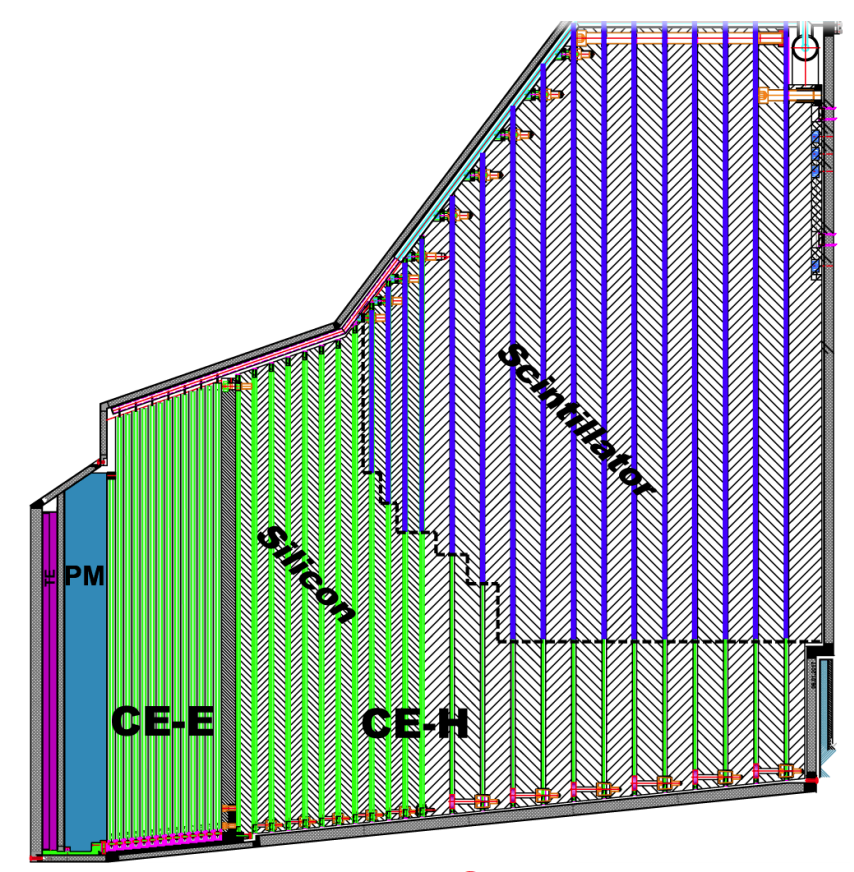
\includegraphics[width=0.8\textwidth]{Figures/HGCAL/TheHGCAL.png}
  \caption[Schematic of the HGCAL.]
  {
    A schematic of the HGCAL's longitudinal structure. 
    The endcap timing layer (TE, purple) is in the front of the HGCAL, 
    nearest to the nominal interaction point.
    A layer of polythene that moderates the flux of neutrons (PM, light blue) 
    also sits in front of the HGCAL.
    The active material of the electromagnetic part of the calorimeter (CE-E) 
    is entirely composed of silicon (green),
    whilst the hadronic part (CE-H) uses a mixture of silicon and plastic scintillator (dark blue)
    as active material.
    Adapted from \cite{HGCAL}.
  }
  \label{fig:hgcal_TheHGCAL}
\end{figure}

\section{Reconstruction}

\subsection{Electromagnetic objects} %TODO add more here, e.g. Artur's plots?

The HGCAL's intrinsic performance measuring the energy of electromagnetic showers 
is modelled using a dedicated simulation 
with pileup corresponding to an average of 200 interactions per bunch crossing. %TODO intrinsic performance means...
Energy deposits in a radius of \SI{26}{mm} around a single unconverted photon 
are summed to estimate the energy resolution, 
which is shown in Figure \ref{fig:hgcal_PhotonReso}. %TODO justify 26mm value
The left plot shows that the resolution is approximately constant as a function of $\eta$, 
and robust against pileup, with only a very small degradation in resolution between PU 0 and PU 200. %this is achieved due to the fine granularity
This intrinsic performance is further demonstrated 
by using this method to reconstruct unconverted photon pairs from simulated \Hgg decays, 
where both photons are contained within the fiducial region of the HGCAL 
and the vertex location is assumed to be known exactly. 
The resulting diphoton mass distribution is shown in Figure \ref{fig:hgcal_DiphotonReso}, 
with resolution of around \SI{1.8}{GeV}.
This value is comparable to the expected resolution of the upgraded CMS barrel calorimeter, 
representing a substantial improvement relative to Run 2, 
where the endcap resolution is significantly worse than the barrel. %TODO quantify this

\begin{figure}[h!]
  \centering
  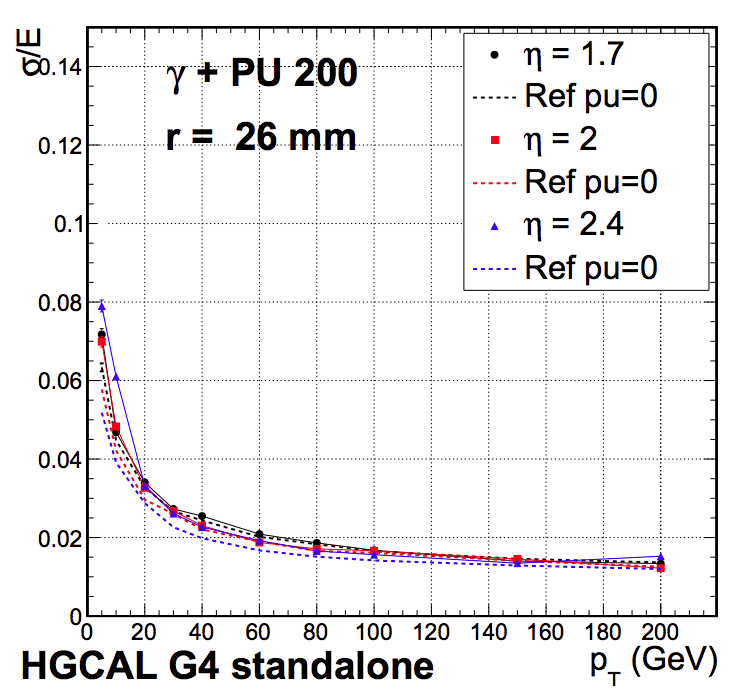
\includegraphics[width=0.6\textwidth]{Figures/HGCAL/SinglePhotonReso.png}
  \caption[HGCAL photon energy resolution.]
  {
    The intrinsic energy resolution for single photons in PU 200. 
    The energy is estimated by summing all deposits within a \SI{26}{mm} radius 
    of the generated particle axis. 
    Figure first shown in from Ref.~\cite{HGCAL}.
  }
  \label{fig:hgcal_PhotonReso}
\end{figure}

\begin{figure}[h!]
  \centering
  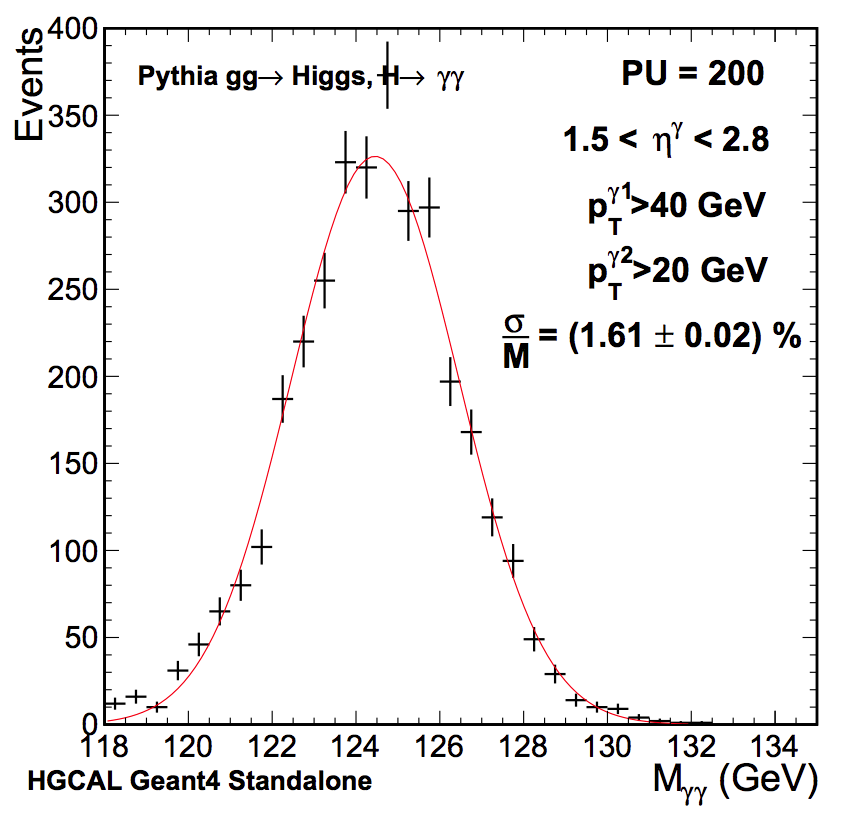
\includegraphics[width=0.6\textwidth]{Figures/HGCAL/HggReso.png}
  \caption[HGCAL diphoton mass resolution.]
  {
    The intrinsic diphoton mass resolution of the HGCAL in simulated \Hgg events 
    where both photons are within the fiducial region of the HGCAL. 
    Figure taken from Ref.~\cite{HGCAL}.
  }
  \label{fig:hgcal_DiphotonReso}
\end{figure}

The HGCAL provides more detailed shower information than existing CMS detectors, 
and it is envisaged that eventually a sophisticated four-dimensional particle flow approach will be used to incorporate as much of this information as possible. 
In the meantime, more straightforward approaches to reconstruction have been developed, 
in order to understand which approaches are feasible and to produce object and physics-level results that demonstrate the potential of the detector. 

%Furthermore, no use is yet made of the intrinsic timing capabilities of the silicon sensors, which will be invaluable in reducing the amount of out-of-time pileup at the HL-LHC. 
The current method begins by clustering hits in each two-dimensional (2D) layer independently, using an imaging algorithm \cite{ClusteringAlgo}.
The algorithm proceeds as follows, and is illustrated in Figure~\ref{fig:hgcal_clustering}:
\begin{enumerate}
  \item Construct an energy density map of all hits above a threshold $E_c$. 
  The threshold value is defined as a function of the noise resolution ($\sigma_{\textrm{noise}}$), which depends on the cell type.
  The density is defined simply as the energy sum of all hits within a critical distance $\delta_c$, 
  whose value is chosen to be similar to the Moli\`ere radius\footnote{The Moli\`ere radius 
  is defined as the radius containing on average 90\% of a shower's total energy deposition}. 
  \item For each hit, calculate the distance to the nearest hit with higher density.
  \item Assign hits with both both density and distance parameters greater than threshold values as cluster centres.
  The density threshold ($\rho_c$) can be defined relative to the maximum density in the event,
  or as a function of the noise resolution.
  The distance threshold is equal to $\delta_c$.
  \item Form clusters by assigning each hit to the same cluster as the nearest hit with higher density.
\end{enumerate}

\begin{figure}[h!]
  \centering
  \begin{subfigure}{0.292\textwidth}
    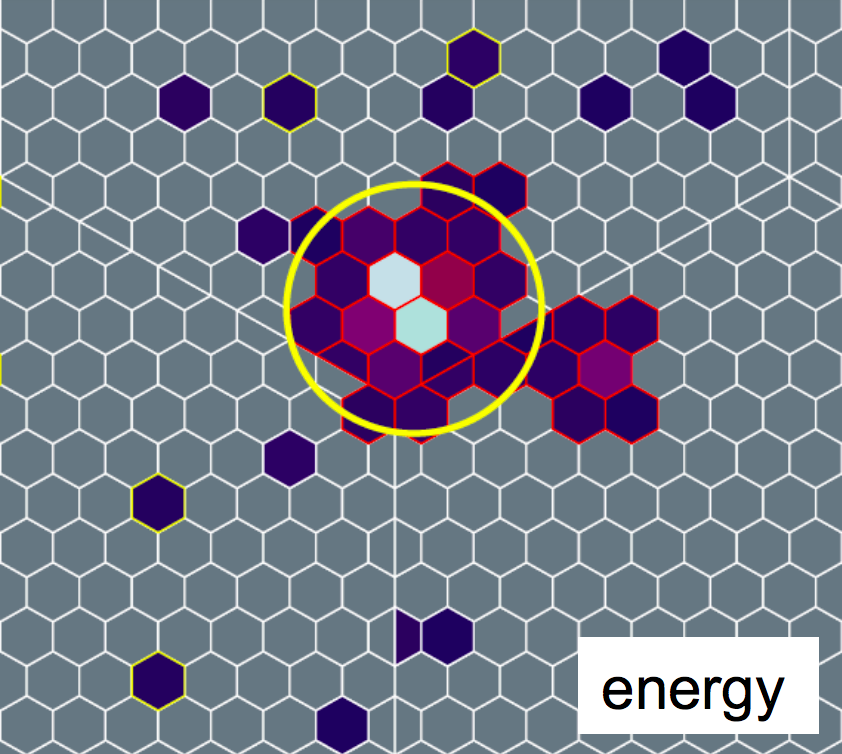
\includegraphics[width=\textwidth]{Figures/HGCAL/ClusteringAlgo_Energy.png}
    \caption{Energy}
  \end{subfigure}
  \begin{subfigure}{0.292\textwidth}
    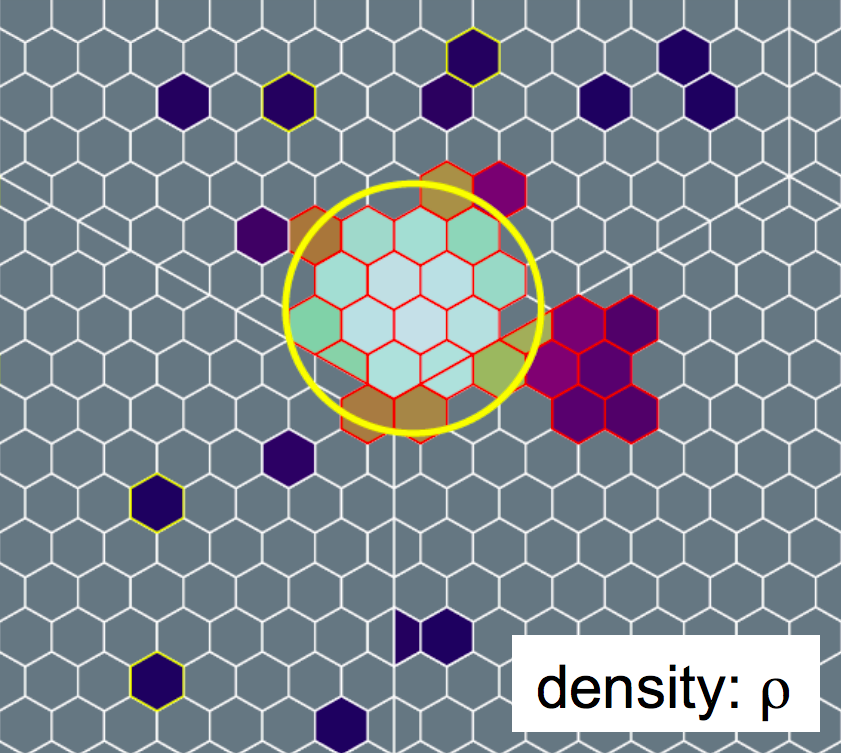
\includegraphics[width=\textwidth]{Figures/HGCAL/ClusteringAlgo_Density.png}
    \caption{Density, $\rho$.}
  \end{subfigure}
  \begin{subfigure}{0.3\textwidth}
    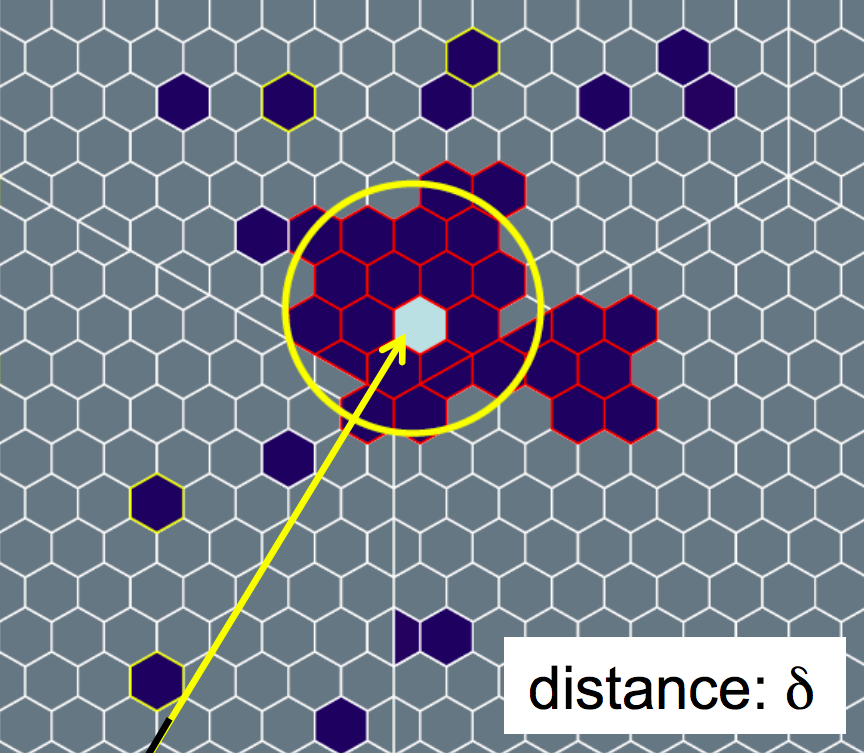
\includegraphics[width=\textwidth]{Figures/HGCAL/ClusteringAlgo_Distance.png}
    \caption{Distance, $\delta$.}
  \end{subfigure}
  \caption[Illustration of the imagine algorithm used for HGCAL layer clustering.]
  {
    Illustration of the procedure used to form layer clusters for electromagnetic objects in the HGCAL.
    The event considered is a single photon with $\pt\,=\,\SI{35}{GeV}$.
    The colour scale represents only the difference between hits, and is in arbitrary units.
    The yellow circle indicates the size of the Moli\`ere radius
    and the yellow arrow points to the hit chosen as a cluster centre.
    It can be seen that many hits in a genuine cluster have a high density, 
    whereas all but one will have a low distance to the nearest higher energy hit;
    requiring high values of both these parameters is therefore an appropriate way to define a cluster.
  }
  \label{fig:hgcal_clustering}
\end{figure}

There are therefore several parameters in the process which can be optimised: $E_c$, $\delta_c$, and $\rho_c$.
To form a suitable object on which to optimise, a more realistic object must be formed.
Therefore the 2D clusters, or layer clusters, produced are associated together in depth to form so-called multiclusters. 
An axis is defined by the highest energy 2D cluster, then any layer clusters within a certain distance of this axis are added to the multicluster.
Using this procedure with sensible parameters, an unconverted photon will have almost all of its energy contained within a single multicluster.
Optimisation can then be performed by minimising the energy resolution of unconverted photons simulated at a range of \pt values.
%It is anticipated that this two-step process could be improved by performing 3D clustering directly, but this remains to be studied in detail. 

Finally, electromagnetic objects are formed using a superclustering procedure very similar to the one utilised in Run 2, 
where showers which have been spread out in the $\phi$ direction by the magnetic field are collected together.
To perform this step, multiclusters are used as inputs to the existing Run~2 algorithm~\cite{PhotonReco}; no re-optimisation is performed.
Despite this, high \pt photons reconstructed in this way in have a resolution of below 2\%, 
not far from the intrinsic resolution values shown in Figure~\ref{fig:hgcal_PhotonReso}.
This method of electromagnetic object reconstruction was used for all the physics results in Ref~\cite{HGCAL}, 
including the study described in Section\ref{sec:hgcal_physics}.

Electrons defined in this way are used to test the ability of the HGCAL 
to discriminate between signal (\Zee) and background (QCD multijet) processes. 
Lateral and longitudinal shower shape variables, 
along with tracking information, are used as inputs to a BDT classifier. 
Two examples are shown in Figure~\ref{fig:hgcal_electronID}: 
the longitudinal development of the shower is indicated by the layer 
at which 10\% of the total energy in the CE-E has been deposited, 
and the lateral spread of the shower evaluated using the pseudorapidity difference 
between the electron multicluster and the extrapolated track.
For both variables, the distributions are robust to the increase in pileup 
and show good discrimination between the signal and background processes.
For a 95\% signal efficiency, the background efficiency is 1\% 
for electrons with $\pt\,>\,\SI{20}{GeV}$, comparable to the Run 2 value. %TODO check Run 2 value
An improvement in performance is seen when the lateral and longitudinal shape variables 
are added to a classifier using solely track information, 
demonstrating the value of the HGCAL granularity to the object identification.

\begin{figure}[h!]
  \centering
  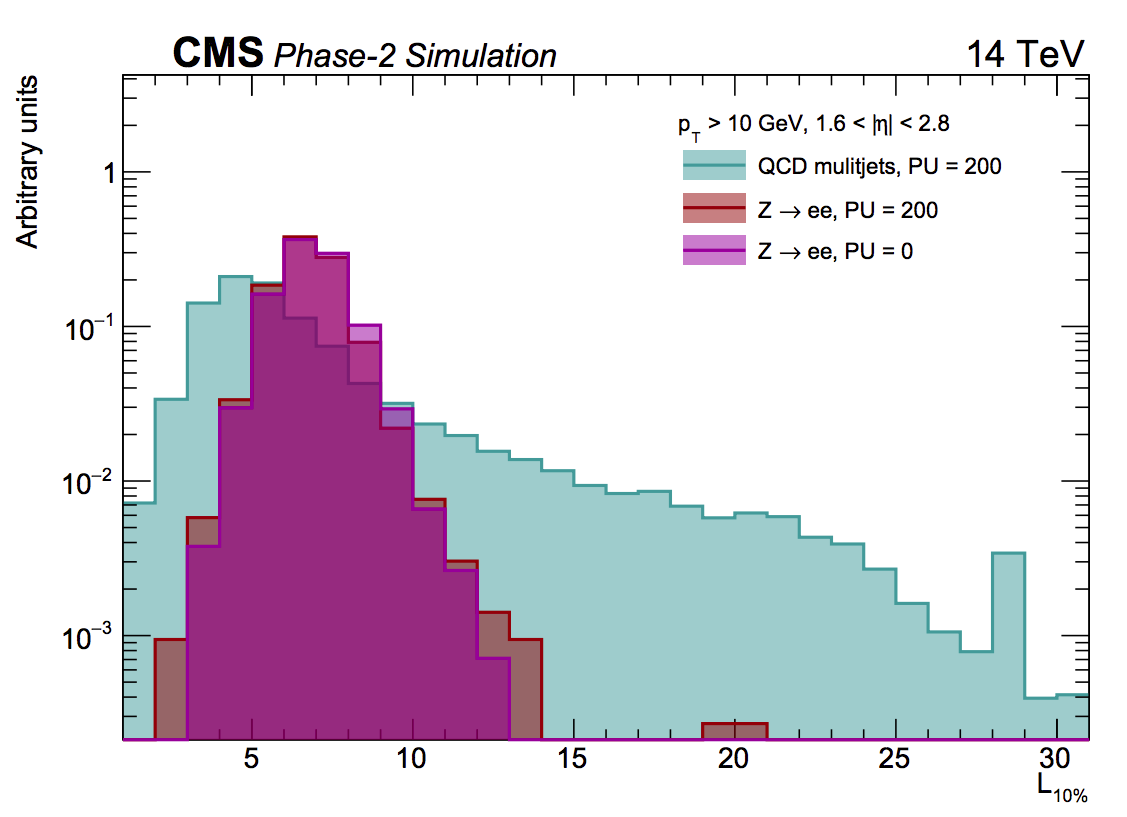
\includegraphics[width=0.7\textwidth]{Figures/HGCAL/electronIDlon.png}
  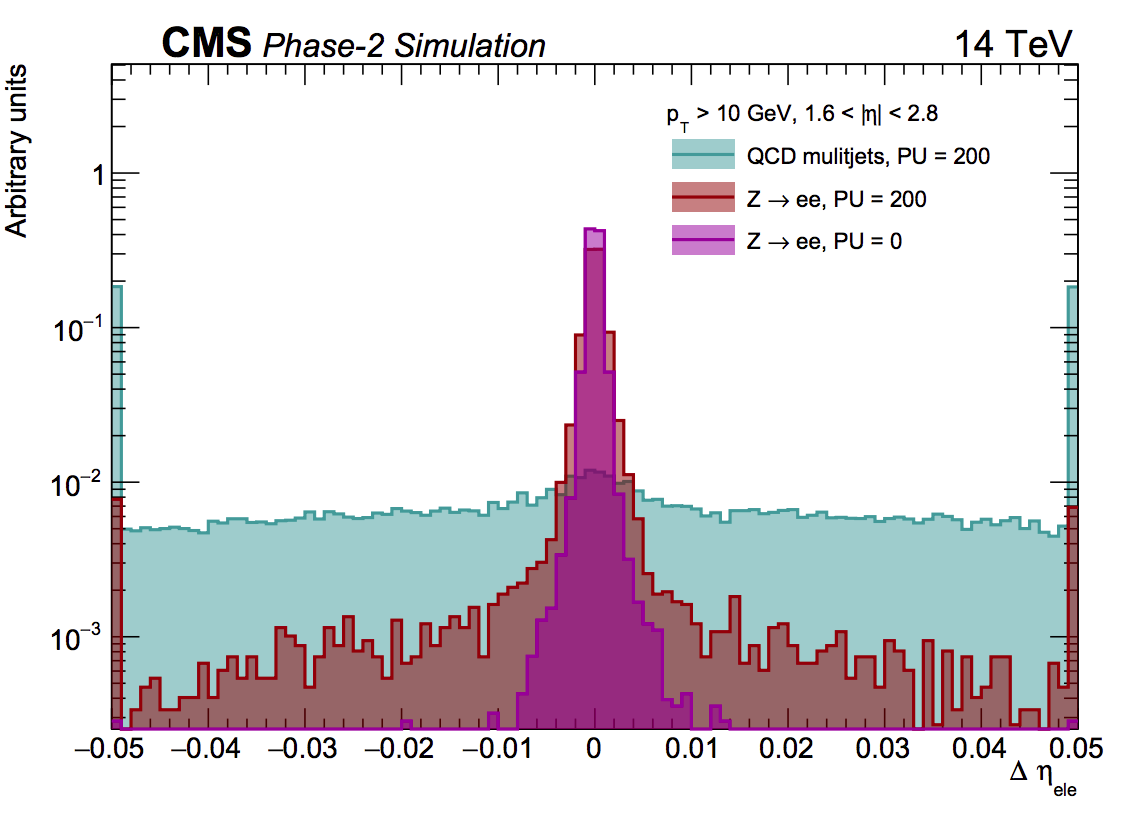
\includegraphics[width=0.7\textwidth]{Figures/HGCAL/electronIDlat.png}
  \caption[Distributions of electron shower shape variables.]
  {
    Shower shape variables used for electron identification.
    The longitudinal development of the shower is indicated by the upper plot, 
    which shows the layer at which 10\% of the total energy in the CE-E is deposited.
    The lower plot shows the pseudorapidity difference between the electron multicluster
    and the extrapolated electron track, which is a measure of the lateral spread of the shower.
    Figures taken from Ref.~\cite{HGCAL}.
  }
  \label{fig:hgcal_electronID}
\end{figure}

\subsection{Hadronic objects}

The multiclustering procedure is not found to work sufficiently well for hadronic showers.
This is due to the fact that hadronic showers are less well-contained, and also have more variation in transverse and longitudinal structure than electromagnetic showers.
Instead, single hadrons were reconstructed using a so-called megaclustering procedure, where layer clusters within a truncated cone are combined to form the object. 
For these more dispersed hadronic showers, the resolution substantially improves once the contribution of pileup is subtracted.
The pileup subtraction was implemented by removing the total energy of a similar cone randomly rotated in $\phi$. 
The energy resolution for a single pion with $\pt\,=\,\SI{25}{GeV}$ before and after the subtraction is shown in Figure \ref{fig:hgcal_SingleMegacluster}. 
The megaclustering algorithm is shown to yield adequate energy resolution of around 20\%. 
It is also robust against pileup; Figure~\ref{fig:hgcal_MegaclusterVsPt} shows the modest worsening between PU 0 and PU 200 that decreases quickly as a function of \pt.
This method of reconstruction is not yet incorporated in the central CMS reconstruction software.
For the physics results in Ref~\cite{HGCAL}, a realistic truth-information-driven approach was instead used for hadronic objects.

\begin{figure}[h!]
  \centering
  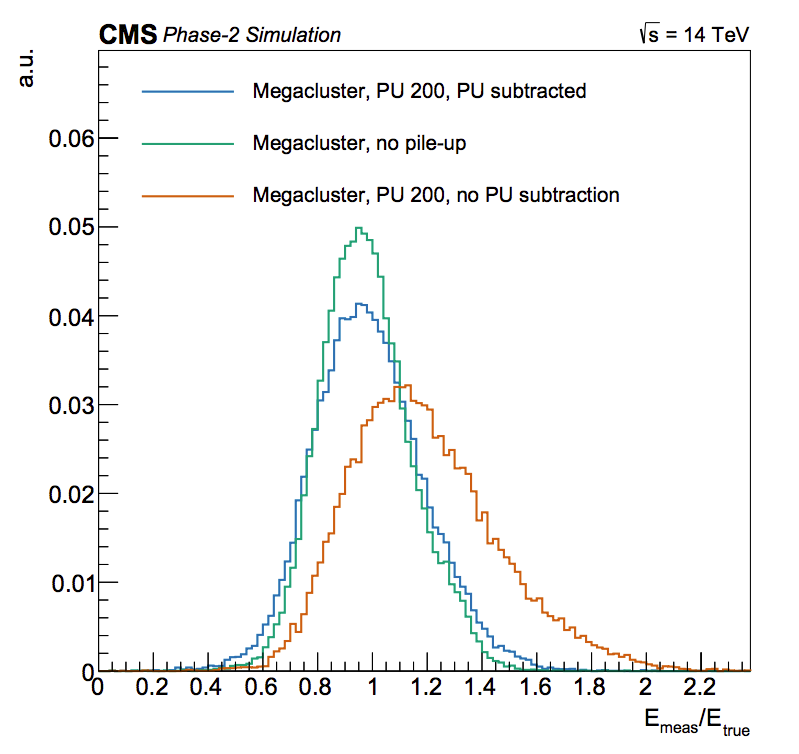
\includegraphics[width=0.65\textwidth]{Figures/HGCAL/SingleMegacluster.png}
  \caption[HGCAL pion energy response.]
  {
    The distribution of the energy resolution for single $\pt\,=\,\SI{25}{GeV}$ pions 
    reconstructed using the megaclustering algorithm, 
    before and after pileup subtraction. 
    Figure taken from Ref.~\cite{HGCAL}.
  }
  \label{fig:hgcal_SingleMegacluster}
\end{figure}

\begin{figure}[h!]
  \centering
  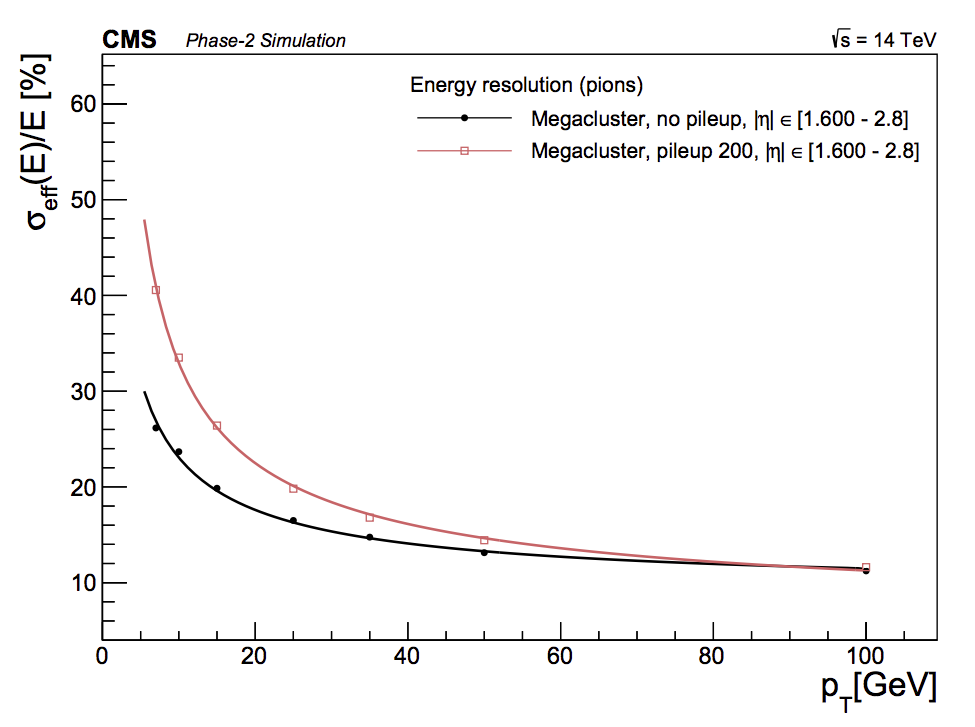
\includegraphics[width=0.7\textwidth]{Figures/HGCAL/MegaclusterVsPt.png}
  \caption[HGCAL pion energy resolution as a function of \pt.]
  {
    The mean energy resolution for single $\pt\,=\,\SI{25}{GeV}$ pions 
    reconstructed using the megaclustering algorithm, after pileup subtraction, 
    as a function of \pt. 
    Figure taken from Ref.~\cite{HGCAL}.
  }
  \label{fig:hgcal_MegaclusterVsPt}
\end{figure}

\subsection{Future development}
The reconstruction methods described above are preliminary and designed only to show the potential performance of the HGCAL subdetector.
There are a wide range of possibilities that will be explored before the eventual installation of the HGCAL.
Firstly, it is possible to extend the 2D clustering algorithm to three dimensions, enabling the construction of multicluster-like objects in one step.
This could potentially improve performance by including correlations between layers and including the longitudinal shower shape, 
rather than treating each layer as independent.
Furthermore, the image-like data produced by the HGCAL is well-suited to the use of machine learning algorithms, particularly those based on neural networks (NNs).
It is likely that eventually the initial pattern recognition step identifying showers will use NNs, and this is already under study.

Secondly, as mentioned above, the CMS particle flow algorithm has not yet been optimised to include all of the new information provided by the upgraded detector.
So far all studies have focussed on the calorimeter system alone; dedicated integration of tracking information, 
probably with an iterative approach, will bring substantial improvements.
This has already been demonstrated by the effectiveness of the particle flow approach in Runs~1 and 2~\cite{ParticleFlow}.

Finally, there is the exciting possibility of performing event reconstruction in four dimensions using timing information.
Both the upgraded ECAL and the HGCAL will provide precise timing information for showers, 
which will be used both for rejecting out-of-time pileup and for the separation of overlapping and adjacent showers.
In addition, the timing information from the MIP timing detector brings many new possibilities. 
It enables the four-dimensional reconstruction of vertices and tracks, 
which has already been shown to improve the vertex identification in \Hgg events at PU 200 from 40\% to 80\% \cite{MTD}.
The added benefit of fully integrating the timing information into the particle flow algorithm in a coherent way remains to be seen.

\section{Physics performance in the \Hgg decay channel}
\label{sec:hgcal_physics}
The performance of the HGCAL and the reconstruction techniques developed for its use 
are tested by evaluating their impact on CMS physics analyses.
In this section, a study of the impact on the CMS \Hgg analysis is described;
the diphoton channel will continue to be very important for characterising the Higgs boson's 
properties at the HL-LHC.
Rather than repeating the analysis in full, 
specific aspects of the analysis which will be affected by the HGCAL upgrade are investigated.

In Run 2, the sensitivity of the \Hgg analysis is driven by barrel-barrel diphoton pairs.
The effect of the HGCAL greater acceptance (to $|\eta|=3$) relative to the current ECAL endcaps
(to $|\eta|=2.5$) is to increase the number of available diphotons by approximately 12\%.
Furthermore, the diphoton mass resolution in the endcap is found to be very similar 
to that in the barrel.
This is an improvement upon the Run~2 endcap, 
which has significantly worse resolution than the barrel, 
and also increases the usefulness of the increased forward acceptance.

A more substantial benefit of the HGCAL upgrade 
will be the ability to separate quark-initiated jets from jets which originate from gluon emission.
This is illustrated in a study of the ggH and VBF production modes in the \Hgg decay channel, 
using events simulated under HL-LHC conditions with the upgraded CMS detector.
In the Run~2 analysis, the so-called dijet BDT is used to discriminate between ggH and VBF
using photon and jet kinematic variables.
Here, the possibility of exploiting the granularity of the HGCAL 
by using jet shape variables as BDT inputs in addition to the kinematic variables is explored.

Jets initiated by gluons tend to have lower \pt values and be more dispersed than quark-initiated jets, 
which are relatively highly collimated and contain fewer particles. 
Therefore variables relating to the jet shapes can be used to discriminate between the two.
Since jets in ggH events tend to be gluon-initiated, 
and the VBF jets quark-initiated, 
this can in turn provide discrimination between the two production processes.

The impact of the HGCAL is evaluated by comparing the performance of two different BDTs.
Three jet shape variables are used to construct a BDT referred to as the jet shape BDT.
A second BDT, known as the dijet BDT, uses additional kinematic variables including those of the photons; 
its inputs are identical to the dijet BDT used in the Run~2 analysis 
(see Chapter~\ref{chap:categorisation} for details), but with the three jet shape variables added.
The same training procedure as that used in the Run~2 analysis was followed, 
where the VBF events are treated as signal, with the ggH as background.
The performance of the two classifiers is illustrated below in Figure \ref{fig:hgcal_VBFvsGGH}.
In each case, a receiver operating characteristic (ROC) curve is constructed.
The ROC curve shows the selection efficiency for signal VBF and background ggH events 
for all values of the BDT output score.
The area under the ROC curve is used a measure of the BDT performance; 
the area is unity for perfect discrimination between signal and background, 
and equals one half if the BDT has no discriminating power.
The area under the ROC curve is 0.71 for the jet shape BDT, and 0.79 for the dijet BDT.
For comparison, the value for the Run 2 dijet BDT was 0.75.
This demonstrates that the additional information provided by the HGCAL translates directly
into an improvement at the analysis level.

\begin{figure}[h!]
  \centering
  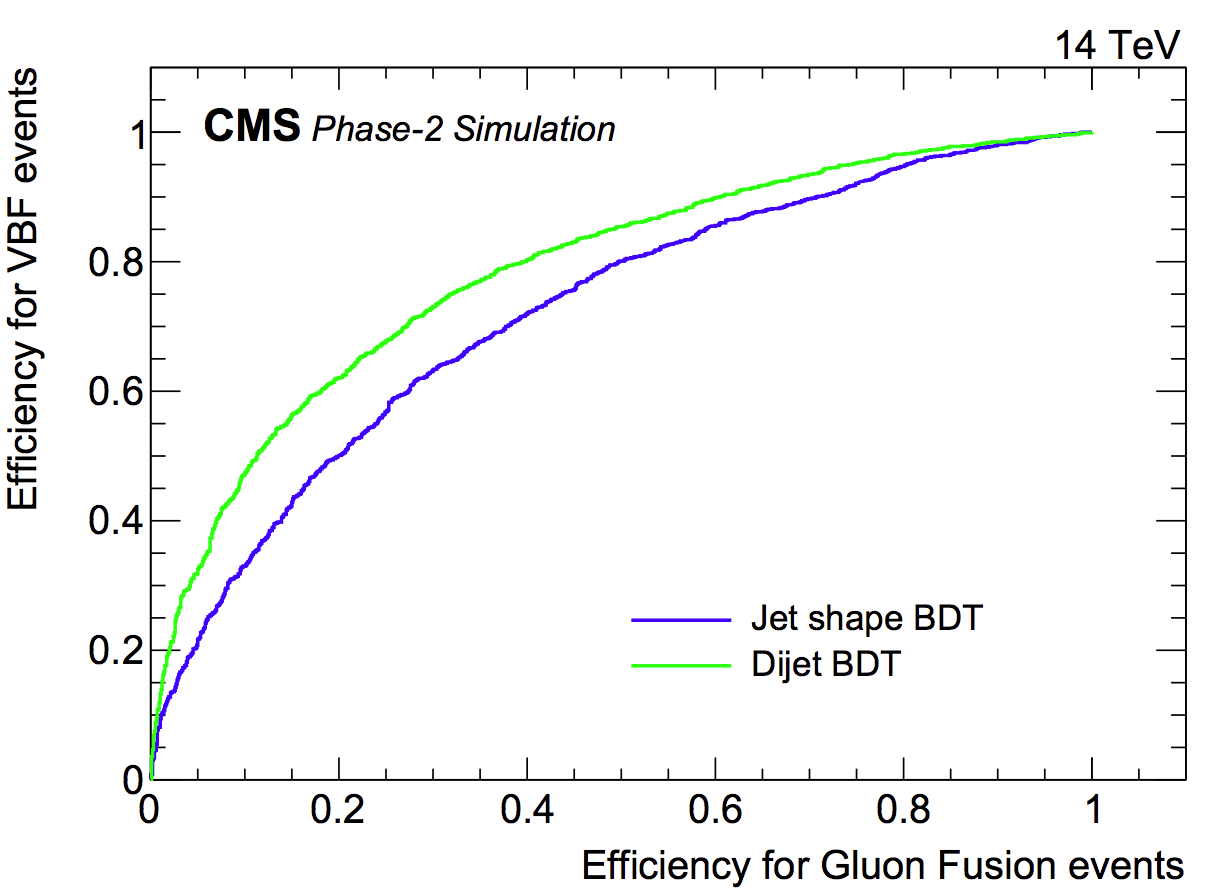
\includegraphics[width=0.8\textwidth]{Figures/HGCAL/VBFvsGGH.png}
  \caption[VBF and ggH selection efficiencies for two BDTs.]
  {
    The selection efficiency for VBF and ggH events for two different BDTs. 
    Figure taken from Ref.~\cite{HGCAL}.
  }
  \label{fig:hgcal_VBFvsGGH}
\end{figure}

Separately, another BDT is trained to reduce the amount of background entering analysis categories.
The VBF events are treated as signal, trained against prompt-prompt, 
prompt-fake and fake-fake \Hgg backgrounds.
This classifier uses only the kinematics of the the two photons as inputs. 
It is less powerful than the Run~2 equivalent 
because not all of the inputs used in the Run~2 version are available.
These include the photon identification score, 
the mass resolution estimates, and the vertex probability estimate.

A 2D scan was used to choose cut values on both the dijet and background BDTs, 
and generate the working points in Table \ref{tab:hgcal_yields}.
The working points were chosen to maximise the total expected significance, 
using the simple metric of the sum in quadrature of the 
the ratio of signal events to the square root of signal plus background events
for each working point~\cite{Asymptotic}.
The number of signal events selected, the fraction of ggH and VBF events, 
and the background per GeV are shown.
Also included is a Run~2 working point, 
consisting of all the events entering the analysis' three VBF tags, for comparison.

%TODO check these numbers
\begin{table}
  \centering
  \begin{tabular}{ r | c |  c |  c |  c }
  \multirow{2}{*}{Event Categories} &\multicolumn{3}{c|}{SM 125 GeV Higgs boson expected signal} & Bkg \\
    &  Total & ggH & VBF & per GeV \\
  \hline
  WP 0 &            750   &  25.4 \%  &  74.6 \%  &  678  \\
  WP 1 &            1275  &  35.9 \%  &  64.1 \%  &  876  \\
  WP 2 &            1926  &  45.8 \%  &  53.2 \%  &  1353 \\
  Summed WP &       3951  &  38.7 \%  &  61.3 \%  &  2907 \\
  Run 2 summed WP & 3878  &  42.0 \%  &  58.0 \%  &  1984 \\
  \end{tabular}
  \caption[Signal and background yields for a VBF \Hgg analysis with the upgraded CMS detector.]
  {
    The signal and background yields for three working points, and the sum thereof.
    The dijet BDT cut is varied, with a fixed cut on the background BDT.
    Number of events given is for \SI{3000}{\fbinv} of collected data. 
    The Run~2 WP contains the sum of selected events in all three VBF categories, extrapolated to \SI{3000}{\fbinv}.
    Table taken from Ref.~\cite{HGCAL}.
  }
  \label{tab:hgcal_yields}
\end{table}

These results show that performance comparable to that in Run~2 
is achieved despite the increase in pileup.
The background numbers are slightly higher than in Run~2, 
but it is expected that this could be reduced by a classifier using further photon quality variables.

\section{Beam tests}

To validate the design of the HGCAL and ensure its behaviour is well-modelled by simulation, 
beam tests have been conducted at both CERN and Fermilab in 2016 and 2017. 
Prototype silicon modules representative of those in both the CE-E and CE-H were built, 
with plastic scintillator tiles modified from an existing detector 
developed by the CALICE collaboration~\cite{CALICE}.
At Fermilab, the available electron beams were of relatively low energy (up to \SI{32}{GeV}), 
and so a test configuration with thickness of around $\SI{15}{X_0}$ was used.
A set of sixteen silicon modules, arranged in sixteen layers, were used.
At CERN, energies of up to \SI{250}{GeV} were available but with only eight modules.
The chosen setup therefore comprised eight layers placed between 5 and $\SI{27}{X_0}$.

Comparisons to simulation of the measured electron energy resolution 
and shower shape are shown in Figure~\ref{fig:hgcal_BeamTest}.
The variable E1/E7 is defined as the ratio of the energy in the most energetic cell (E1) 
to the sum of the energies of the most energetic cell and its six surrounding cells (E7);
this indicates the lateral extent of the shower.
Also shown is the relative energy resolution for a range of energy values, 
using both the CERN and Fermilab setups.
In both cases, excellent agreement is observed between data and simulation;
observed distributions match those predicted by simulation to within 5\%. 
These beam test results are particularly important because 
they constitute the first demonstration that the HGCAL behaves as predicted by simulation.

Furthermore, additional tests confirm the expected intrinsic timing capabilities of the silicon sensors, 
with the timing resolution measured to be less than \SI{30}{\pico\second}.
The timing performance of the silicon was also measured to be a function of S/N only, 
meaning it does not degrade with increasing radiation exposure. 

\begin{figure}[h!]
  \centering
  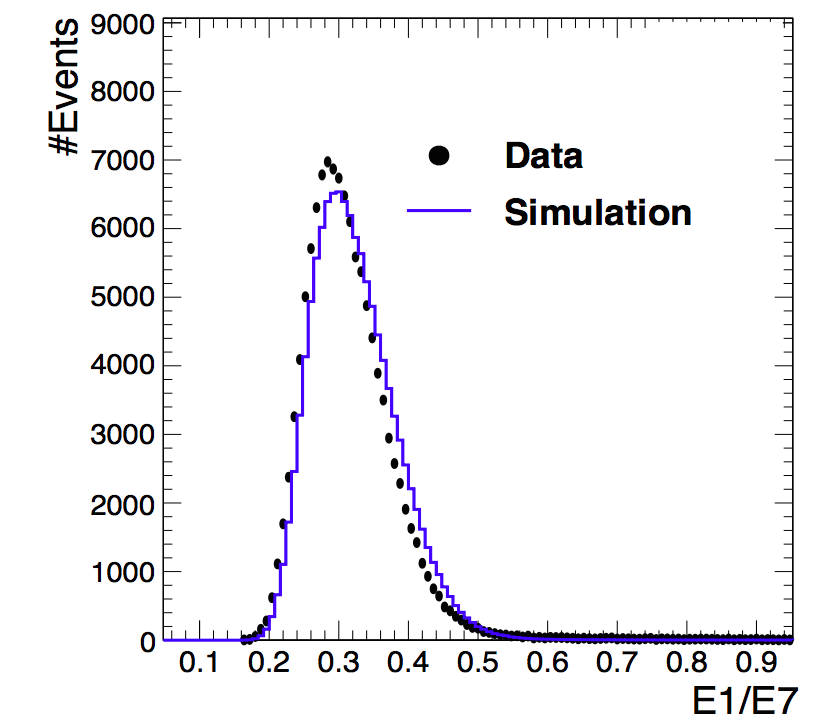
\includegraphics[width=0.7\textwidth]{Figures/HGCAL/BeamTestShape.png}
  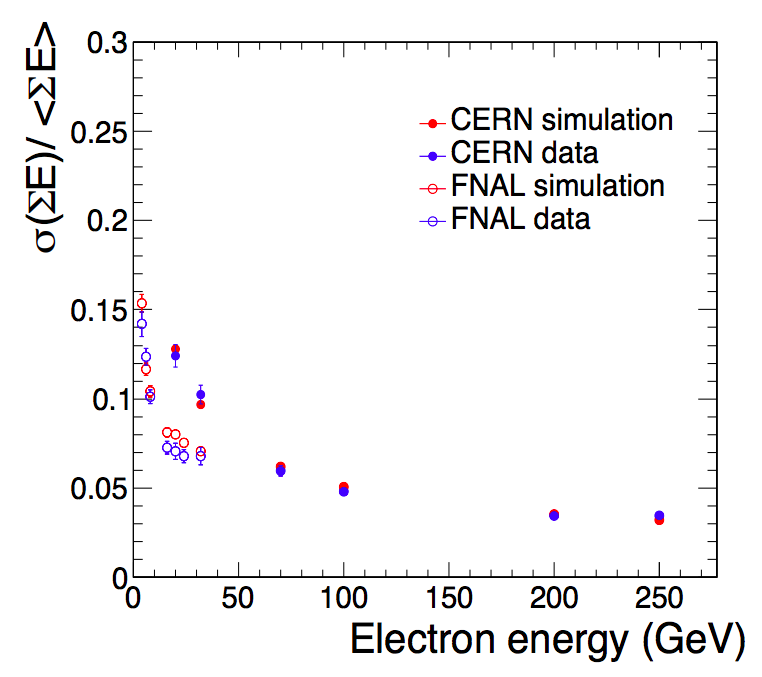
\includegraphics[width=0.7\textwidth]{Figures/HGCAL/BeamTestEnergy.png}
  \caption[Comparison of data and simulation in HGCAL beam tests.]
  {
    The upper plot shows the distribution of the energy ratio E1/E7 (defined in the text) 
    for \SI{100}{GeV} electrons using the CERN beam test setup.
    Data points are shown in black and the blue histogram represents the simulation.
    The lowe plot shows the relative electron energy resolution as a function of energy, 
    for both the CERN (solid circles) and Fermilab (hollow circles) setups.
    Simulated points are shown in red, with data points in blue.
    Figures taken from Ref.~\cite{HGCAL}.
  }
  \label{fig:hgcal_BeamTest}
\end{figure}
